%%%%%%%%%%%%%%%%%%%%%%%%%%%%%%%%%%%%%%%%%%%%%%%%%%%%%%%%%%%%%%%%%%%%%%%%
%                                                                      %
%     File: Thesis_Background.tex                                      %
%     Tex Master: Thesis.tex                                           %
%                                                                      %
%     Author: Andre C. Marta                                           %
%     Last modified :  2 Jul 2015                                      %
%                                                                      %
%%%%%%%%%%%%%%%%%%%%%%%%%%%%%%%%%%%%%%%%%%%%%%%%%%%%%%%%%%%%%%%%%%%%%%%%

\chapter{State of the Art}
\label{chapter:stateoftheart}


To reflect the current use cases of GPUs and the efforts made in the pursuit of improving the performance and minimizing the energy consumption of them, this chapter provides an overview of the architecture of modern GPUs, with a brief specialization on the AMD GNC architecture. It also presents what kinds of power savings techniques are currently being employed in the existent hardware in the market and a review of the literature related to this subject. Furthermore, an overview of power and performance models is provided, highlighting how does the performance and power requirements are affected by the workload 


%%%%%%%%%%%%%%%%%%%%%%%%%%%%%%%%%%%%%%%%%%%%%%%%%%%%%%%%%%%%%%%%%%%%%%%%
\section{General Purpose Computing on GPUs}
\label{section:gpuarch}

A GPU is a highly parallel programmable processor, that is built to perform the same instruction on a set of data, belonging to the category of processors of \textit{Single Instruction Multiple Threads} - SIMT. When referring to GPUs, it is still common to be talking about their graphics capabilities, however, more and more programs are taking advantage of their highly parallel architecture to accelerate applications. The use of GPUs in general programming commonly referred to as GPGPU - General Purpose Graphical Processing Unit was first led by the development of CUDA by NVIDIA and OpenCL by Khronos Group. CUDA and OpenCL are both parallel computing platforms and application programming interface (API) that allows developers to create GPU-accelerated applications, where the computation can be divided between the CPU and GPU. However, the first versions of these frameworks treated the GPU as a slave device, providing a set of directives that allow the CPU (master device) to transfer data, synchronize and control the GPU.  Though, to take full advantage of the GPU architecture and create a true heterogeneous system, the CPU and GPU collaborate more efficiently. This lead, in 2012, the HSA Foundation to propose the Heterogeneous System Architecture HSA \cite{hwu_heterogeneous_2015} framework that acts as an intermediary low-level API to provide improved coordination and communication for heterogeneous computing systems.  More recently, AMD introduced the Radeon Open Computing platform (ROC) \cite{noauthor_radeonopencompute/rocm_2019}. ROC, like CUDA and OpenCL, provides a set of tools that allow developers to create heterogeneous applications. The added benefits of ROC are that it is built on top of the HSA runtime API and that exposes the framework in a wider set of programming frameworks like OpenCL, HC++, and HIP.

The development of improved frameworks and programming methodologies are making GPUs the prime tool to accelerate big-data applications and deep learning algorithms. GPUs can outperform CPUs in both throughput and energy efficiency. In this section, it will be provided a general overview of the GPU architecture, followed by an exploration of architectural techniques that are being employed to reduce power consumption and increase the efficiency of these devices.


\subsection{General Overview of GPU Architecture}
The architecture of the GPU can be roughly divided into computation and memory components. The computation part is composed of the vertex shader, the rendering engine, and the RISC processors. The vertex shader and rendering engine are inserted on the graphics pipeline and are not generally used on GPGPU applications. The RISC processors are responsible for the GPU programmable calculations, and depending on the manufacturer, can be called streaming multiprocessors (SMs) in NVIDIA GPUs \cite{nvidia_cuda_nodate} or computing units (CU) in AMD GPUs \cite{amd_amd_nodate}. To support thousands of concurrent threads simultaneously, each CU is made up of hundreds of execution units. Every CU has a statically allocated register file, where each thread can reserve a physical part of it \cite{jing_energy-efficient_2013}. To enable concurrent execution of multiple threads in a single CU and allow low-overhead context switch, modern GPUs provide a large register file, where the context of all active threads can be stored. For reference, in the AMD GNC architecture, each CU has 49152 (32-bit) registers.

In terms of memory, both the AMD and the NVIDIA GPU present a 3 level hierarchy system: a global memory, accessible by all processors units (generally referred as video memory); a shared memory associated with each SM or CU, accessible by the processing units of that SM or CU; and a set of read-only caches for constants and textures.

A GPU from AMD will be used to conduct the experimental part of this dissertation. For that reason, a more in-depth analysis of the architecture and framework from this manufacturer will be provided and the terminology used by it will be adopted. However, the presented work is independent of the hardware and terminology itself.

\subsection{AMD Graphics Core Next}

The AMD Graphics Core Next (GCN) \cite{amd_radeons_nodate}  architecture includes both the GPU microarchitecture as well as the instruction set of the processor unit. It was first released in 2012 and it is already in its fifth iteration with the codename Vega. The Vega microarchitecture is based on a multiprocessor chip with an array of 64 RISC SIMT processors called Compute Engine (CE). Respectively, each CE is constituted by 64 Next Compute Units (NCU), performing a total of 4096 stream processors. also called Compute Units. The interface between the GPU and the Host is done throw the Peripheral Compute Interconnect Express (PCIe). Figure \ref{fig:Vega10arch} represents the logical organization of a Vega GPU. 

\begin{figure}[!htb]
  \begin{subfigmatrix}{2}
    \subfigure[Chip block diagram, example with 4 CEs]{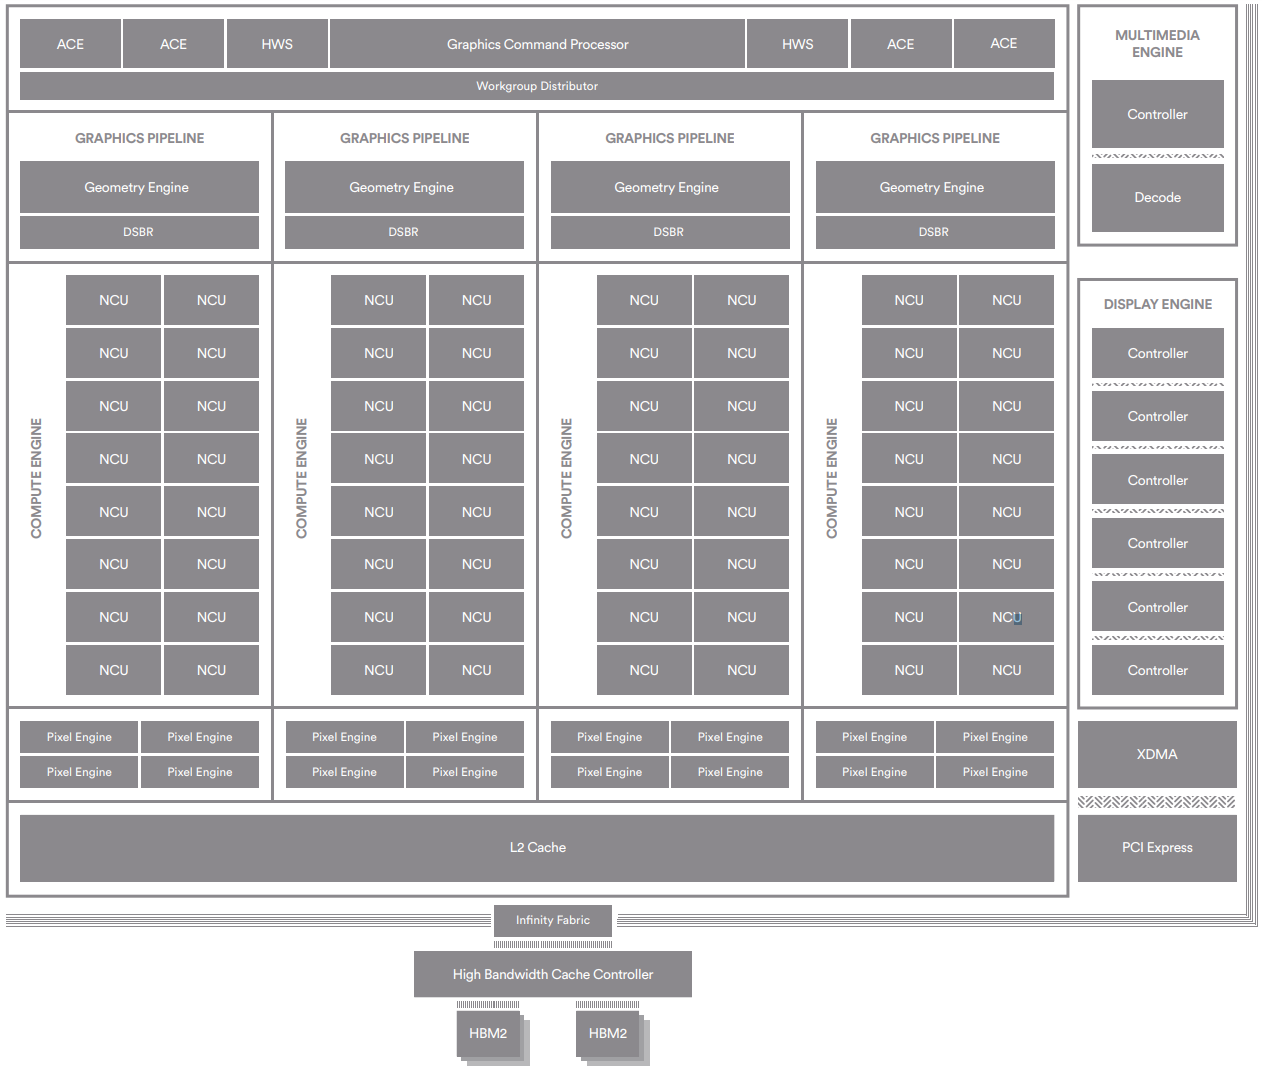
\includegraphics[width=0.7\linewidth]{Figures/StateArt/Vega10_microarchitecture.png}}
    \subfigure[NCU]{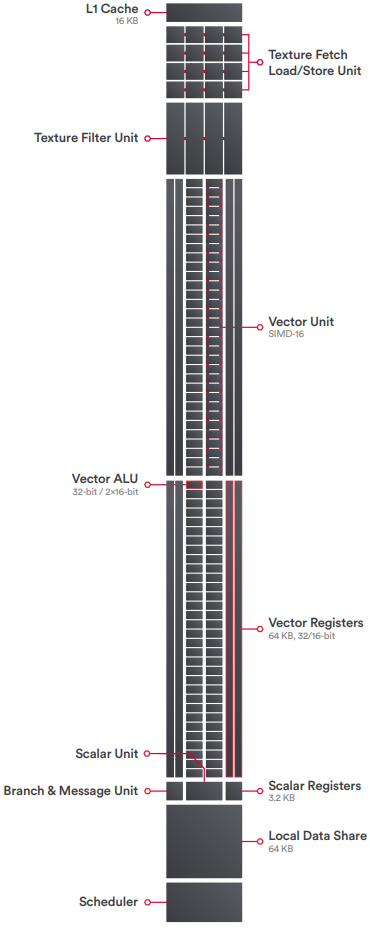
\includegraphics[width=0.29\linewidth]{Figures/StateArt/NCU.png}}
  \end{subfigmatrix}
  \caption{AMD's Graphics Core NExt logical Organization.}
  \label{fig:Vega10arch}
\end{figure}

In the fifth iteration of the GNC microarchitecture, AMD introduced a new memory hierarchy and support for High-Band Memory 2 (HBM2). In a conventional memory arrangement, the registers of each processing element pull data from a set of L1 caches, that, in turn, access the global L2 cache. Finally, the L2 cache system provides access to the GPU's video memory. This arrangement implies that the video memory has the entire working set of data and resources, in order to provide high-bandwidth and low-latency access to data. However, in complex graphical scenes or while working GPGPU applications with large datasets, the total video memory may not be big enough to store all the data. In the Vega microarchitecture, by utilizing a  High-Bandwidth Cache Controller (HBCC), AMD made possible to utilize the local video memory like a last-level cache. In this arrangement, when a missing piece of data is not currently stored in the local memory, the GPU can pull from the host, just the necessary page memory. In this setup, instead of the GPU stalling, while the entire missing resource is copied from the host throw the PCIe bus, it just needs to wait for the smaller page memory to be transferred, resulting in significantly decreased memory access times. The GPGPU applications take great advantage of this memory hierarchy since it enables the use of bigger datasets than the ones that could fit in video memory.

In the development of the work of this dissertation, a Radeon Vega Frontier Edition GPU is used. Table \ref{tab:gpusepcs} summarizes the most important specifications of the architecture of this device.

\begin{table}[!htb]
    \renewcommand{\arraystretch}{1.2} % more space between rows
    \centering
        \begin{tabular}{lc}
            \multicolumn{1}{c}{\textbf{}} & \multicolumn{1}{l}{\textbf{Radeon™ Vega Frontier Edition}} \\ \hline
            Base Architecture             & Vega GNC                                                   \\
            \#Compute Units               & 64                                                         \\
            \#Stream Processors           & 4096                                                       \\
            GPU Memory Size               & 16 GB                                                      \\
            Thermal Design Power          & 300 W                                                      \\ \hline
        \end{tabular}
    \caption{Characteristics of the used GPU device}
    \label{tab:gpusepcs}
\end{table}

\subsection{Radeon Open Compute platform}

The Radeon Open Compute (ROC) \cite{noauthor_radeonopencompute/rocm_2019} platform provides support for a set of frameworks and tools to allow developers to program and control the AMD GPUs. Figure \ref{fig:rocmplatform} shows the high-level organization of the platform. The platform includes a set of tools that allows developers to access ROC Kernel Driver data. In the following subsections, two of those tools, the ROCM-SMI \cite{noauthor_radeonopencompute/roc-smi_2019} and ROC-Profiler \cite{noauthor_rocm-developer-tools/rocprofiler_2019} tools, used on the development of this work, are described.

\begin{figure}[!htb]
  \centering
  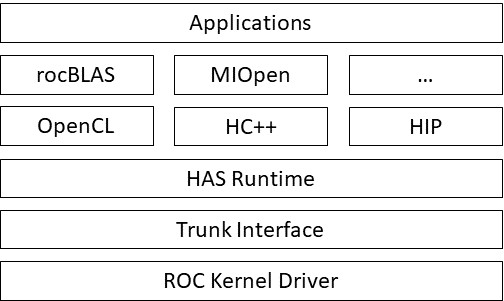
\includegraphics[width=0.5\textwidth]{Figures/StateArt/ROC_stack.jpg}
  \caption{Organization of the ROC platform.}
  \label{fig:rocmplatform}
\end{figure}

\subsubsection{ROCM-SMI}
The ROCm System Management Interface (ROC-SMI) \cite{noauthor_radeonopencompute/roc-smi_2019} is a user-friendly command-line application for manipulating the Radeon Open Compute Kernel (ROCK). The application uses sysfs files to query and manipulate the device kernel using the libsensors library \cite{noauthor_libsensors3:_nodate}. Using it, it is possible to know and control the state of the GPU device.

From the set of query and control directives enabled by ROC-SMI, the following are of particular interest for the topic of this dissertation:

\begin{itemize}
\item \textbf{GPU utilization:} Retrieves the current utilization rates for the device's major subsystems, one value for the processing core and other for the main device memory. These values are computed over a specific time interval that is directly set on the libsensors library. The processing core utilization reflects the percentage of time that the GPU core was being utilized to perform computations whereas the main device memory utilization reflects the times on which the memory was being read or written.

\item \textbf{GPU power}: Retrieves the average power being used by the device. Similarly to the utilization rate, the average power computed over the same time interval, during which, a defined number of power samples are taken.

\item \textbf{Clock rate and voltage level:} Retrieves both the currently applied clock frequency and voltage level to the GPU core and the main device memory. It also displays two tables, the first, showing the 8 pairs of clock frequency and voltage level of the GPU core and the second, showing 4 pairs of the same parameters related to the device memory. These two tables, correspondent to the 8 and 4 performance levels that the device kernel can apply to the GPU core and memory correspondingly.
\end{itemize}

The ROC-SMI interface also allows querying the device temperature, the current fan speed, and the selected performance level.

ROC-SMI, also provides a mechanism to control and change device parameters such as:
\begin{itemize}
\item \textbf{Set clock rate and voltage level:} Set the clock frequency and the voltage level of any of the performance levels of both the GPU core and memory. 
\item \textbf{Set performance level:} Allows the user to select the desired performance level of the GPU core and device memory, disabling the driver automatic performance level management system.
\item \textbf{Reset clock rate and voltage level:} Resets the clock rates and voltage level to the default values.
\end{itemize}

Additionally, the interface allows the user to manually set the fan speed, important to manually guarantee that all the executed tests are performed at the same temperature level.

The versatility and total and independent control of the clock rate and voltage level of the device allowed by ROCM-SMI and the libsensors library was the defining factor for choosing an AMD GPU over the more popular options of NVIDIA. In the development of the work presented in this dissertation, an exploration of the voltage level is undertaken, and only the AMD platform allows for independent control over this variable.

\subsubsection{ROC-Profiler}

The Radeon Open Compute Profiler \cite{noauthor_rocm-developer-tools/rocprofiler_2019} is a profiling and tracing library for applications developed using any of the programming frameworks available on the ROC platform (OpenCL, HC++, HIP) \cite{sun_evaluating_2018}. The library gives access to the performance counters of AMD GPUs, allowing developers to configure the start, stop, read and reset of the physical registers on the microarchitecture that count the number of events (number of instructions per type, cache hits/miss, etc) that the device is performing.

The instrumentation of applications with the API calls to rocprofiler allows for close monitoring of the operations being performed and can give important insights about the relation that the running code as with the results being achieved on the frequency and voltage exploration.


%%%%%%%%%%%%%%%%%%%%%%%%%%%%%%%%%%%%%%%%%%%%%%%%%%%%%%%%%%%%%%%%%%%%%%%%


\section{Dynamic Voltage and Frequency Scaling}
\label{section:dcvf}

The widespread use of GPUs in both supercomputers as on personal machines comes at the cost of a significant increase in the power consumption of the complete system. Whereas a typical modern CPU consumes about 50 to 100W, it is common to see GPUs rounding that value to 200 to 300W of power. With these figures, it is indispensable the use of energy efficiency techniques to try to reduce power consumption.

On any CMOS circuit, the total power consumed is decomposed into the dynamic and static parts. The dynamic power is generated when the transistors flip their stages and correspond to the power of charging and discharging the internal net capacitances. This value is proportional to the frequency that this change occurs. Equation \ref{eq:dynpower} represents the general formu for dynamic power, where \textit{a} represents the utilization factor, \textit{C} the total capacitance of the circuit, \textit{V} the transistors supplied voltage and \textit{f} the operating frequency \cite{gonzalez_supply_1997}.
\begin{equation}
    P_{dynamic} = aCV^2f
    \label{eq:dynpower}
\end{equation}


On their turn, the static part of the power consumption is generated by $P_{leakage}$, $P_{short-circuit}$ and $P_{DC}$ \cite{mei_survey_2016}. The leakage power is independent of the transistors flip, and it represents the flow of electrons that exists between the transistors' source, drain, and gate. The short-circuit power comes from the instantaneous short-circuit connection between the supply voltage and the ground when the transistor flips. Finally, the Direct Current (DC) power corresponds to the power needed for powering the circuit. Equation \ref{eq:cmospower} represents the total power consumption sources.

\begin{equation}
    P_{total} = P_{dynamic} + P_{leakage} + P_{short-circuit} + P_{DC}
    \label{eq:cmospower}
\end{equation}

The total power consumption of a circuit is dominated by the dynamic power, however, with the reduction of the manufacturing size of the transistor seen nowadays, the static power is also contributing heavily \cite{s._hong_modeling_2012} \cite{hong_integrated_2010}. As a common reference, due to the higher height of the dynamic power on the total power consumption, the power used by a circuit changes linearly with the clock frequency and quadratically with the supplied voltage.


By intelligently controlling the clock frequency, the necessary voltage for stable operation of the circuit can also be reduced, leading to power savings. However, the reduction of the operating frequency harms the pic performance of the circuit, so a careful scaling of voltage/frequency needs to be done in run-time. The "on the fly" control of these parameters is called Dynamic Voltage and Frequency Scaling (DVFS). This power management technique allows for an energy efficiency improvement by matching the voltage and frequency of the processor to the utilization that is being given to it.



In general, modern GPU boards have independent control over two pairs of frequency and voltage. Each pair or domain acts on a distinct part of the GPU, intending to maximize the performance or reduce the power consumption. The first domain concerns the GPU core, acting on all CUs, the cache, and the interconnection fabric. The second affects the DRAM chips that compose the video memory. 

The clock frequency is an independent control variable and its change is reflected directly on the performed achieved by the GPU. An increase in the clock frequency of the core results in an improvement of the CU execution speed, while the same change in the memory frequency will increase the DRAM I/O throughput \cite{mei_survey_2016}. The voltage level of each domain is dependent on the clock frequency and is computed based on tests performed by the manufacturer that ensure the correct operation of the circuit, independently of the workload that is being given.

Both AMD and NVIDIA equip their GPUs with complex DVFS systems that choose the most appropriate combination of GPU voltage and frequency for each domain.  In the case of AMD, the GPU core has 8 possible pairs, table \ref{tab:gpucorelevels}, while the GPU memory has only 4, table \ref{tab:gpumemlevels}. Through the use of software like ROC-SMI \cite{noauthor_radeonopencompute/roc-smi_2019} it is possible for the user to input the desired combination of values for each level, allowing for an almost continuously selection of values for the frequency and voltage within the specifications range. For example, on the Vega 10 Frontier Edition used on the experimental work of this thesis, the GPU core frequency can be set between 852 and 1980 MHz and the GPU memory frequency between 167 and 1500 MHz. The voltage is set between the 800 and 1250 mV. As stated before, the major benefit of AMD over NVIDIA's solution is that this manufacturer allows for the override of the automatic computation of the GPU voltage. This difference is of significant importance since it allows finer control of the DVFS values and a more interesting possibility of exploration of the voltage level.

\begin{table}[!htb]
\renewcommand{\arraystretch}{1.2} % more space between rows
\centering
\begin{tabular}{ccc}
\textbf{Level} & \textbf{Frequency {[}MHz{]}} & \textbf{Voltage {[}mV{]}} \\ \hline
0              & 852                          & 800                       \\
1              & 991                          & 900                       \\
2              & 1138                         & 950                       \\
3              & 1269                         & 1000                      \\
4              & 1348                         & 1050                      \\
5              & 1440                         & 1100                      \\
6              & 1528                         & 1150                      \\
7              & 1600                         & 1200                      \\ \hline
\end{tabular}
\caption{GPU Core Levels of Frequency and Voltage of AMD Vega 10 Frontier Edition}
\label{tab:gpucorelevels}
\end{table}

\begin{table}[!htb]
\renewcommand{\arraystretch}{1.2} % more space between rows
\centering
\begin{tabular}{ccc}
\textbf{Level} & \textbf{Frequency {[}MHz{]}} & \textbf{Voltage {[}mV{]}} \\ \hline
0              & 167                          & 800                       \\
1              & 500                          & 900                       \\
2              & 800                          & 950                       \\
3              & 945                          & 1000                      \\ \hline
\end{tabular}
\caption{GPU Memory Levels of Frequency and Voltage of AMD Vega 10 Frontier Edition}
\label{tab:gpumemlevels}
\end{table}




\subsection{Control Mechanism}

\begin{figure}[!htb]
  \centering
  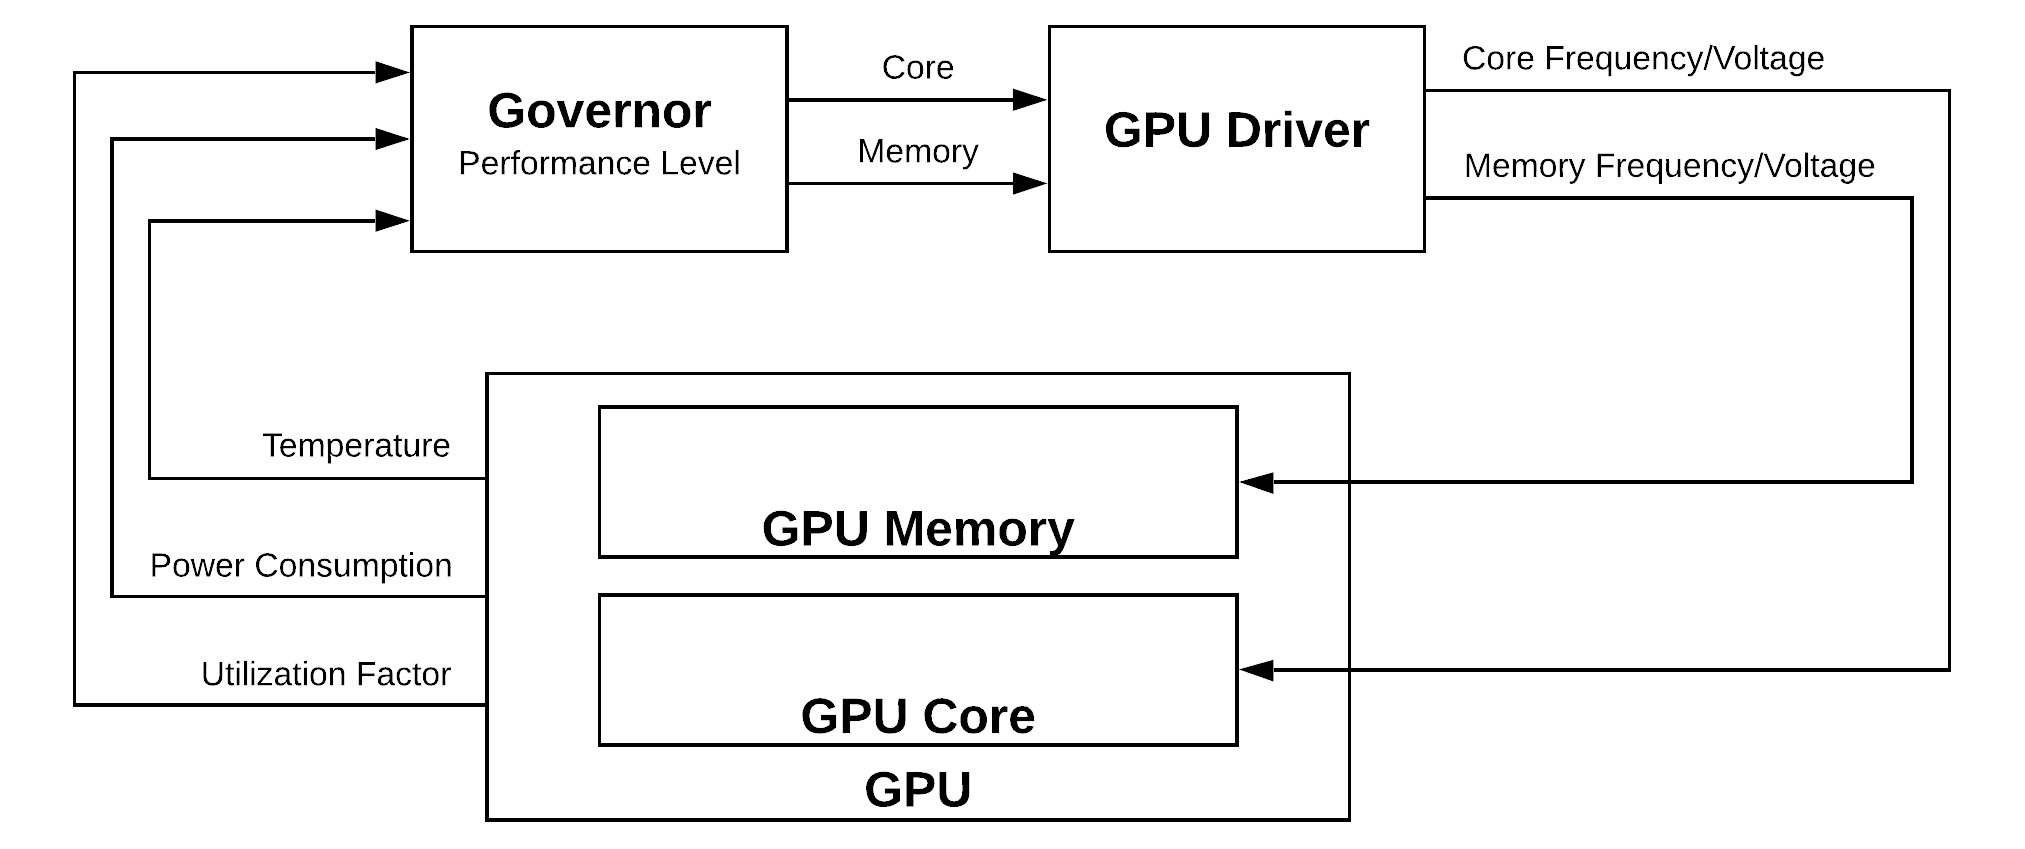
\includegraphics[width=0.75\textwidth]{Figures/StateArt/DVFS.png}
  \caption[Controller]{DVFS control mechanism.}
  \label{fig:DVFSmechanism}
\end{figure}

%Fazer um diagrama todo bonito a mostrar o sistema de realimentação


%talk about CPU

\subsection{Clock splitting techniques}

\subsection{DVFS Optimizations}

%grande margem para fazer tudo, nao optimizado


\subsection{Dynamic Voltage and Frequency Scaling Effects}
https://www.researchgate.net/publication/261725696_A_Survey_of_Methods_For_Analyzing_and_Improving_GPU_Energy_Efficiency




%%%%%%%%%%%%%%%%%%%%%%%%%%%%%%%%%%%%%%%%%%%%%%%%%%%%%%%%%%%%%%%%%%%%%%%%
\section{Models}
\subsection{Power Modeling}
\label{section:powermodels}
\subsubsection{Empirical Methods}
\subsubsection{Statistical Methods}

\subsection{Performance Modeling}
\label{section:powermodels}
\subsubsection{Pipeline Analysis}
\subsubsection{Statistical Methods}
Performance Counters

\section{Related Work}

\section{Summary}


For the early processing units, the dynamic power accounts for the majority of power consumption, but nowadays the static power is also contributing considerably